% !TeX spellcheck = da_DK
\section{Samlet systemtest}
Efter de enkelte blokke er blevet testet og godkendt hver for sig, skal det samlede system testes. Formålet med den samlede systemtest er at kontrollere, hvorvidt systemet overholder de overordnede funktionelle krav jævnfør afsnit \ref{FunkKrav} på side \pageref{FunkKrav}. Der anvendes samme fremgangsmåde for test af det samlede system, som af de øvrige blokke; Først simuleres systemet i LTspice, hvorefter det implementeres og testes.

\subsection{Simulering}
I simuleringen af det samlede system kontrolleres det, som i de øvrige simuleringer, om systemet fungerer med ideelle komponenter. Denne kontrol udføres ved at indsende et sinussignal som inputspænding til systemet, som teoretisk skal aktivere hhv. de enkelte dioder og vibratorerne. Designet af det samlede system ses på \figref{fig:samlet_system}:
\begin{figure}[H]
	\centering
	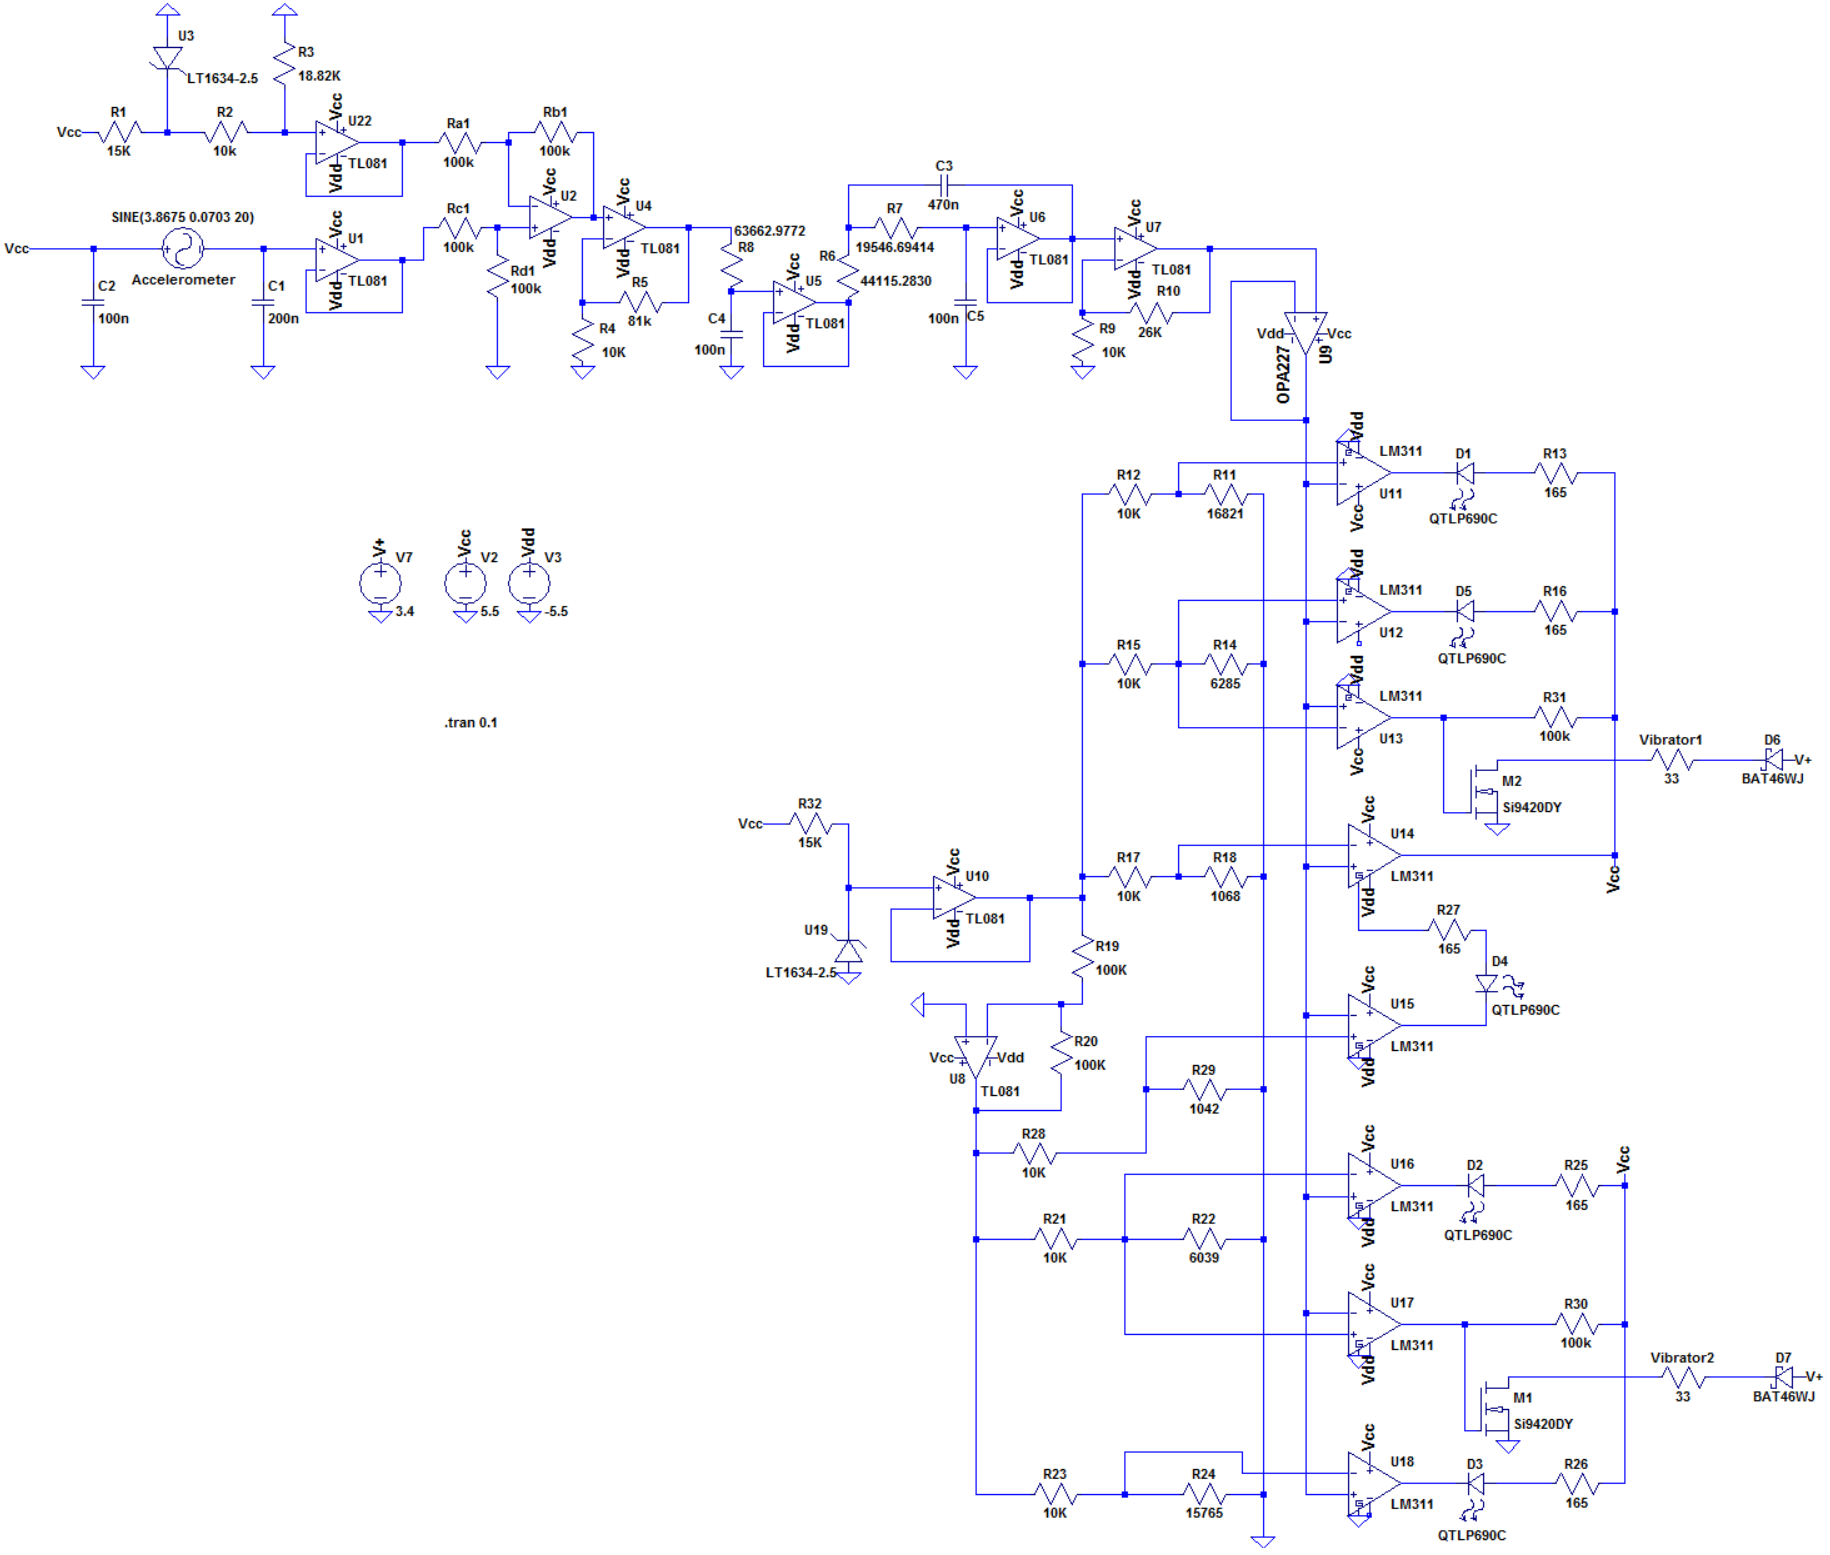
\includegraphics[scale=.38]{figures/cProblemloesning/Samlet_systemUL.PNG}
	\caption{På figuren ses designet af det samlede system.}
	\label{fig:samlet_system}
\end{figure}
\noindent Sinussignalets amplitude udregnes til at være:
\begin{eqnarray}
0.0037 \cdot (\dfrac{(25-13)}{2} + 13) = 0.0703V
\end{eqnarray}
\noindent $0.0037$V er den maksimale spænding fra accelerometret ved $1^{\circ}$ hældning. Dette ganges med $19$, hvilket er midterpunktet for aktivering af en rød diode ($13^{\circ}$ hældning) og mætning af den sidste forstærker ($25^{\circ}$ hældning). Der opnås en amplitude på $0.0703$V. Det kan derved måles, om systemet teoretisk opfylder de overordnede funktionelle krav jævnfør afsnit \ref{FunkKrav} på side \pageref{FunkKrav}.\\
For at simulere systemet, som ses \figref{fig:samlet_system}, er det nødvendigt at foretage nogle basale ændringer i det opstillede system i LTspice, for at en computer kan køre det. Ændringerne omfatter, at blokke, som leverer en uændret spænding, udskiftes med en spændingsforsyning, som leverer denne spændingsværdi. Dermed fjernes nogle operationsforstærkere fra det teoretisk opstillede system, hvorefter computeren kan konfigurere en simulering. Designet med basale ændringer kan ses på \figref{fig:samlet_system}
\begin{figure}[H]
	\centering
	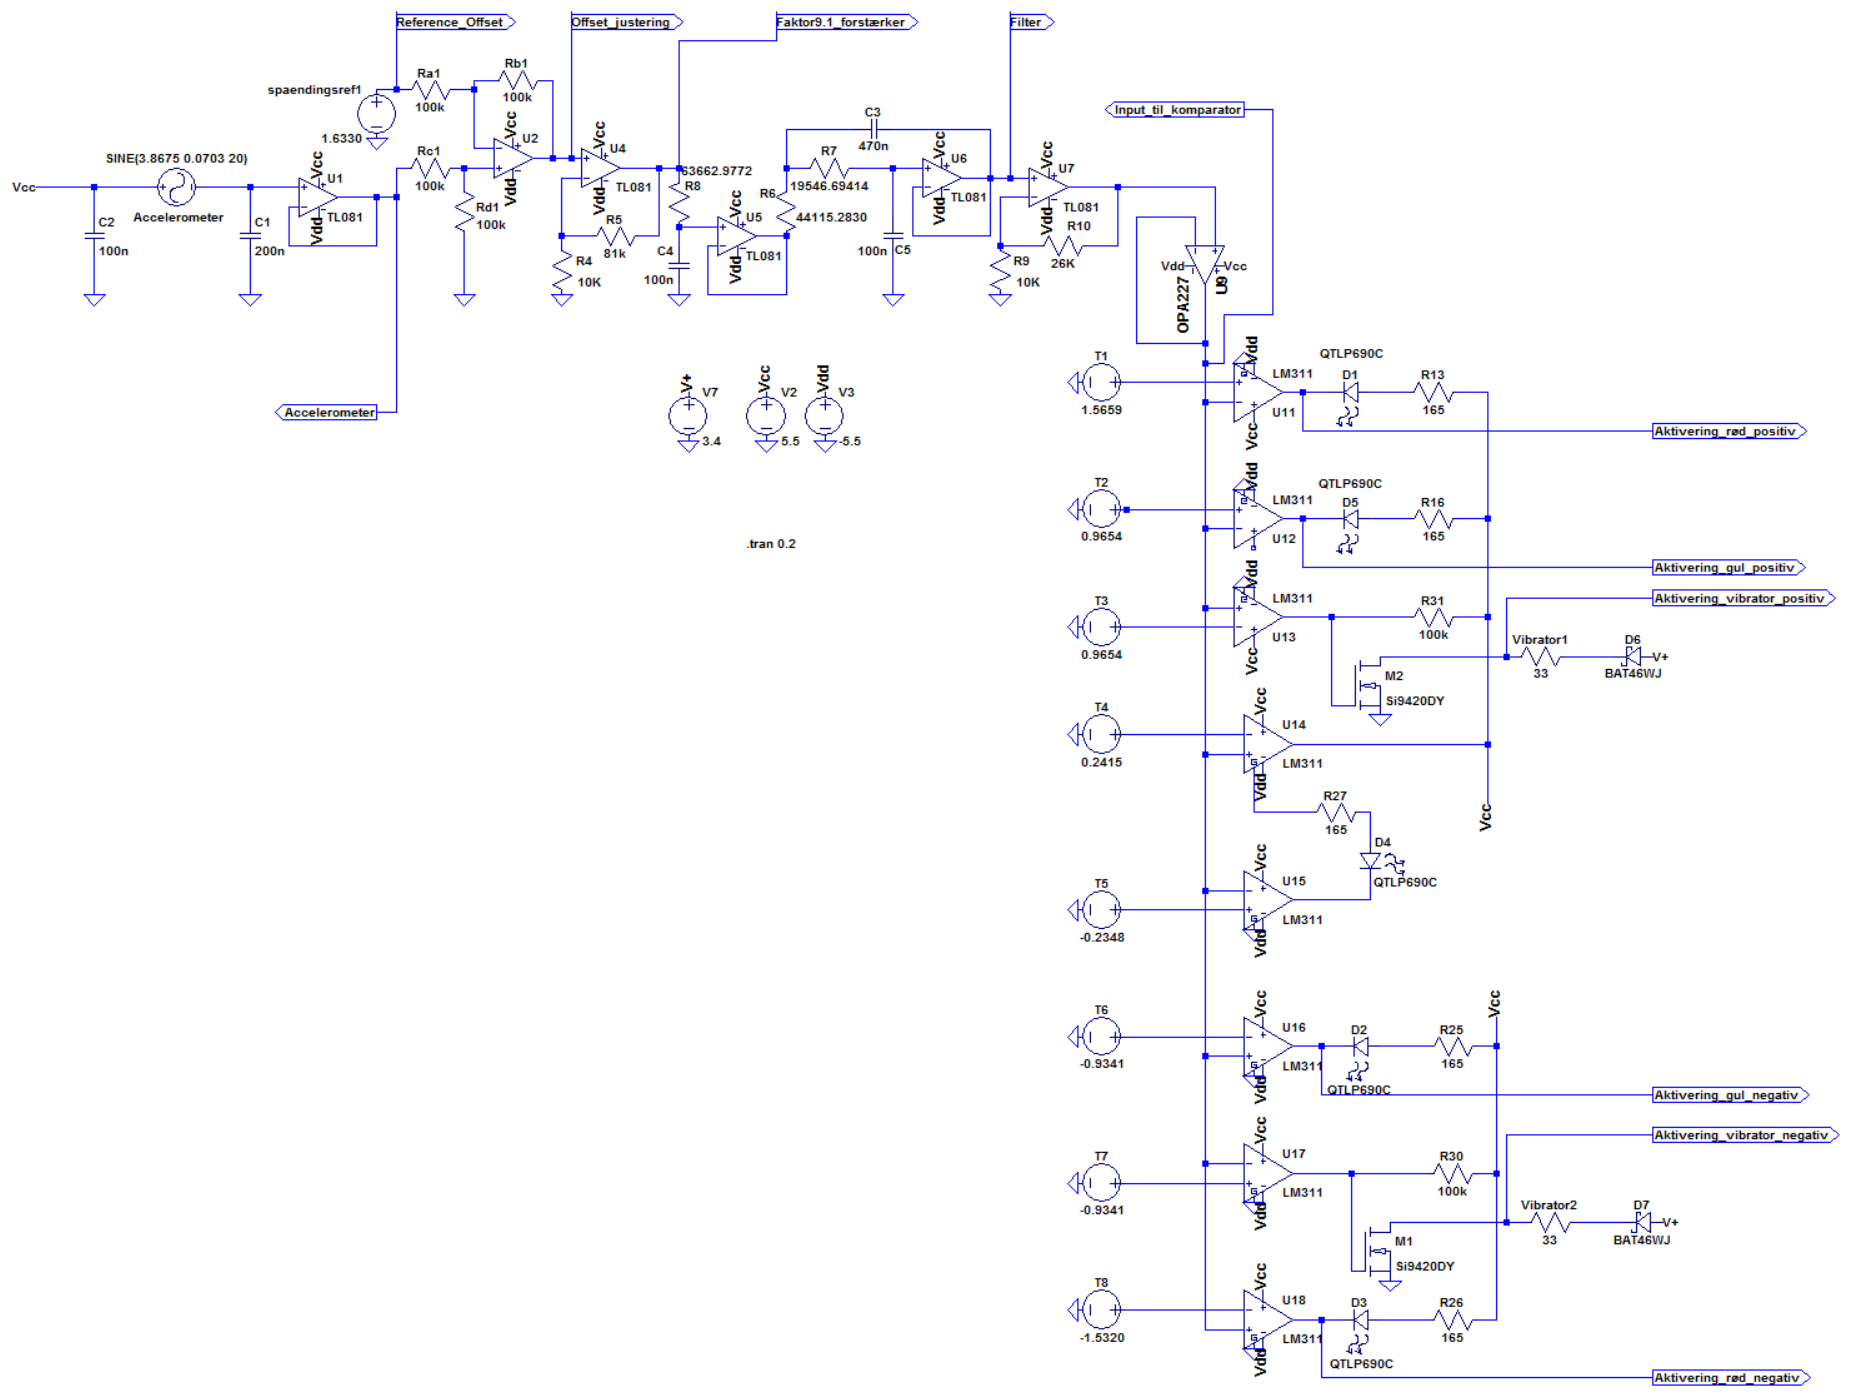
\includegraphics[scale=.38]{figures/cProblemloesning/Samlet_system2_sim.PNG}
	\caption{På figuren ses designet af det forenklede samlede system med labels, der indikerer målepunkterne for de følgende simuleringer. Derved kan blokkenes effekt på signalet følges undervejs i systemet. Referencespændingen til offsetjusteringsblokken er erstattet med en spændingsforsyning på $1.6325$V, hvilket konfigurationen, som før var forbundet her, teroretisk skulle levere. Derudover er hele konfigurationen, som skulle skabe tærskelværdier til komparatorerne, udskiftet med spændingsforsyninger, som leverer den simulerede tærskelværdi i volt til hver komparatorkonfiguration, som er målt i \tableref{Tab:test_reference1} på side \pageref{Tab:test_reference1}.}
	\label{fig:samlet_system}
\end{figure}
\noindent Simuleringen kan herefter foretages. Resultatet fra simuleringen ses på nedenstående figurer.
\begin{figure}[H]
	\centering
	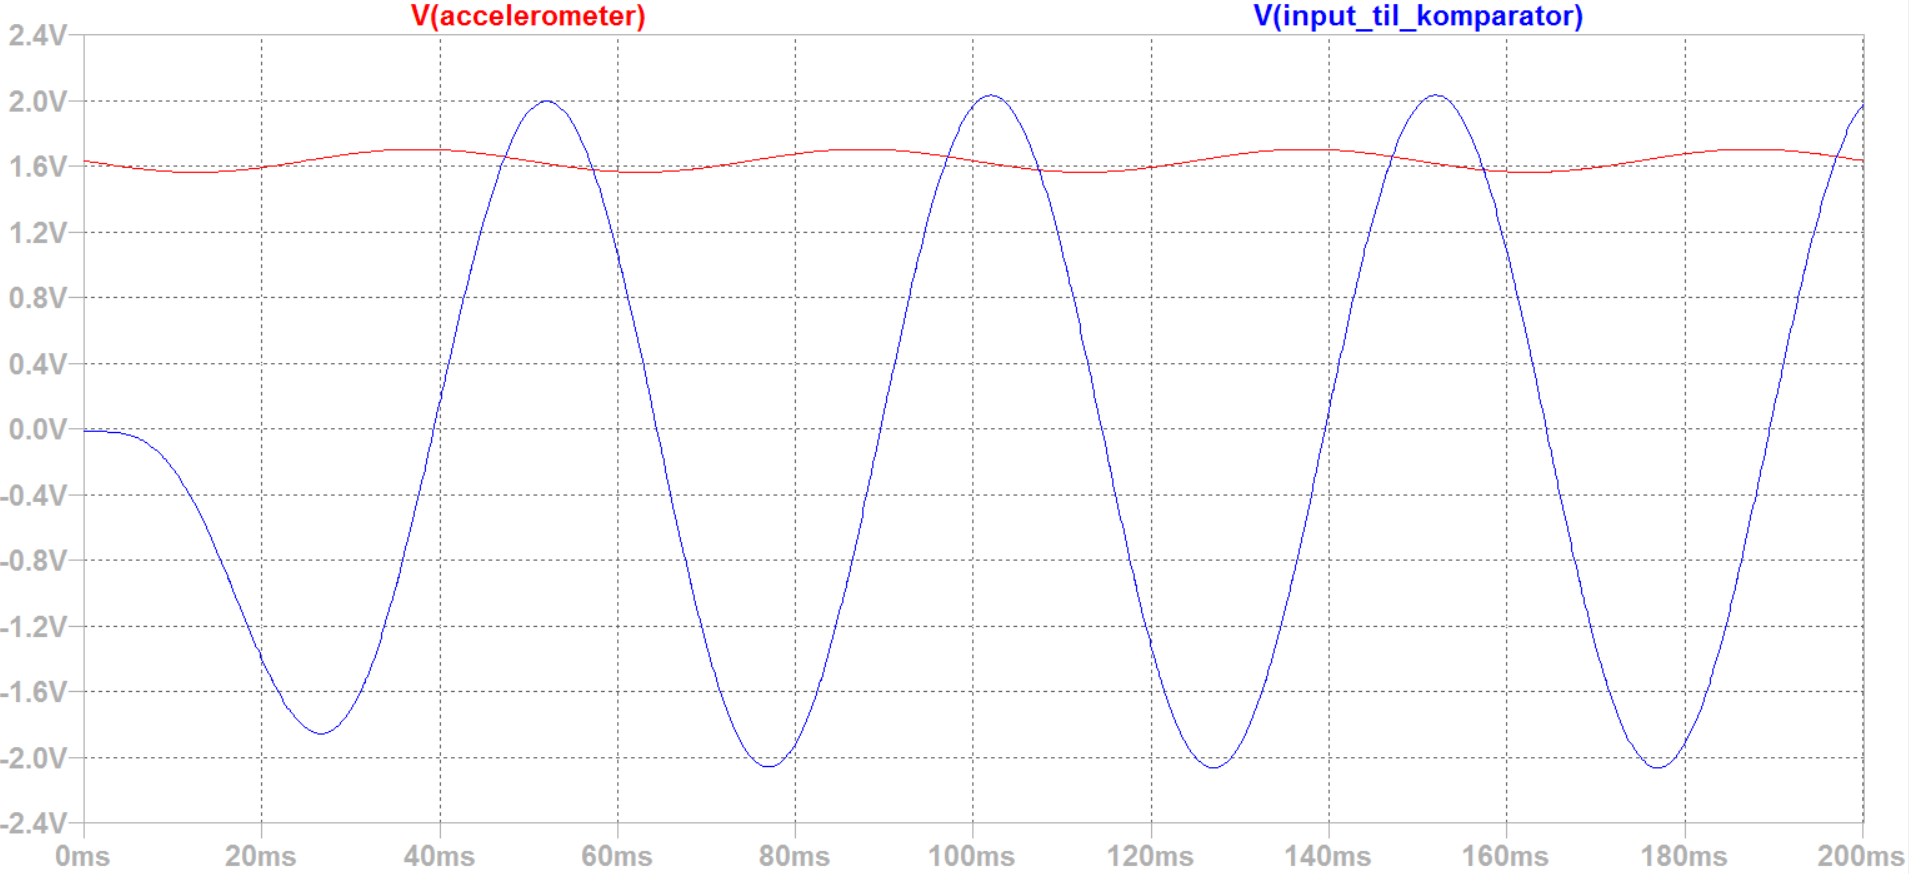
\includegraphics[scale=.3]{figures/cProblemloesning/Samlet_system_sim12.PNG}
	\caption{På figuren ses outputtet fra accelerometret plottet sammen med inputtet til komparatorblokken. Der ses, at signalets offset er blevet justeret, så signalet nu er centreret omkring 0V. Derudover er signalet blevet forstærket to gange og filtreret. Dette ses ved, at amplituden er blevet forstørret og frekvensen er forskudt.}
	\label{fig:samlet_system_sim1}
\end{figure}
\begin{figure}[H]
	\centering
	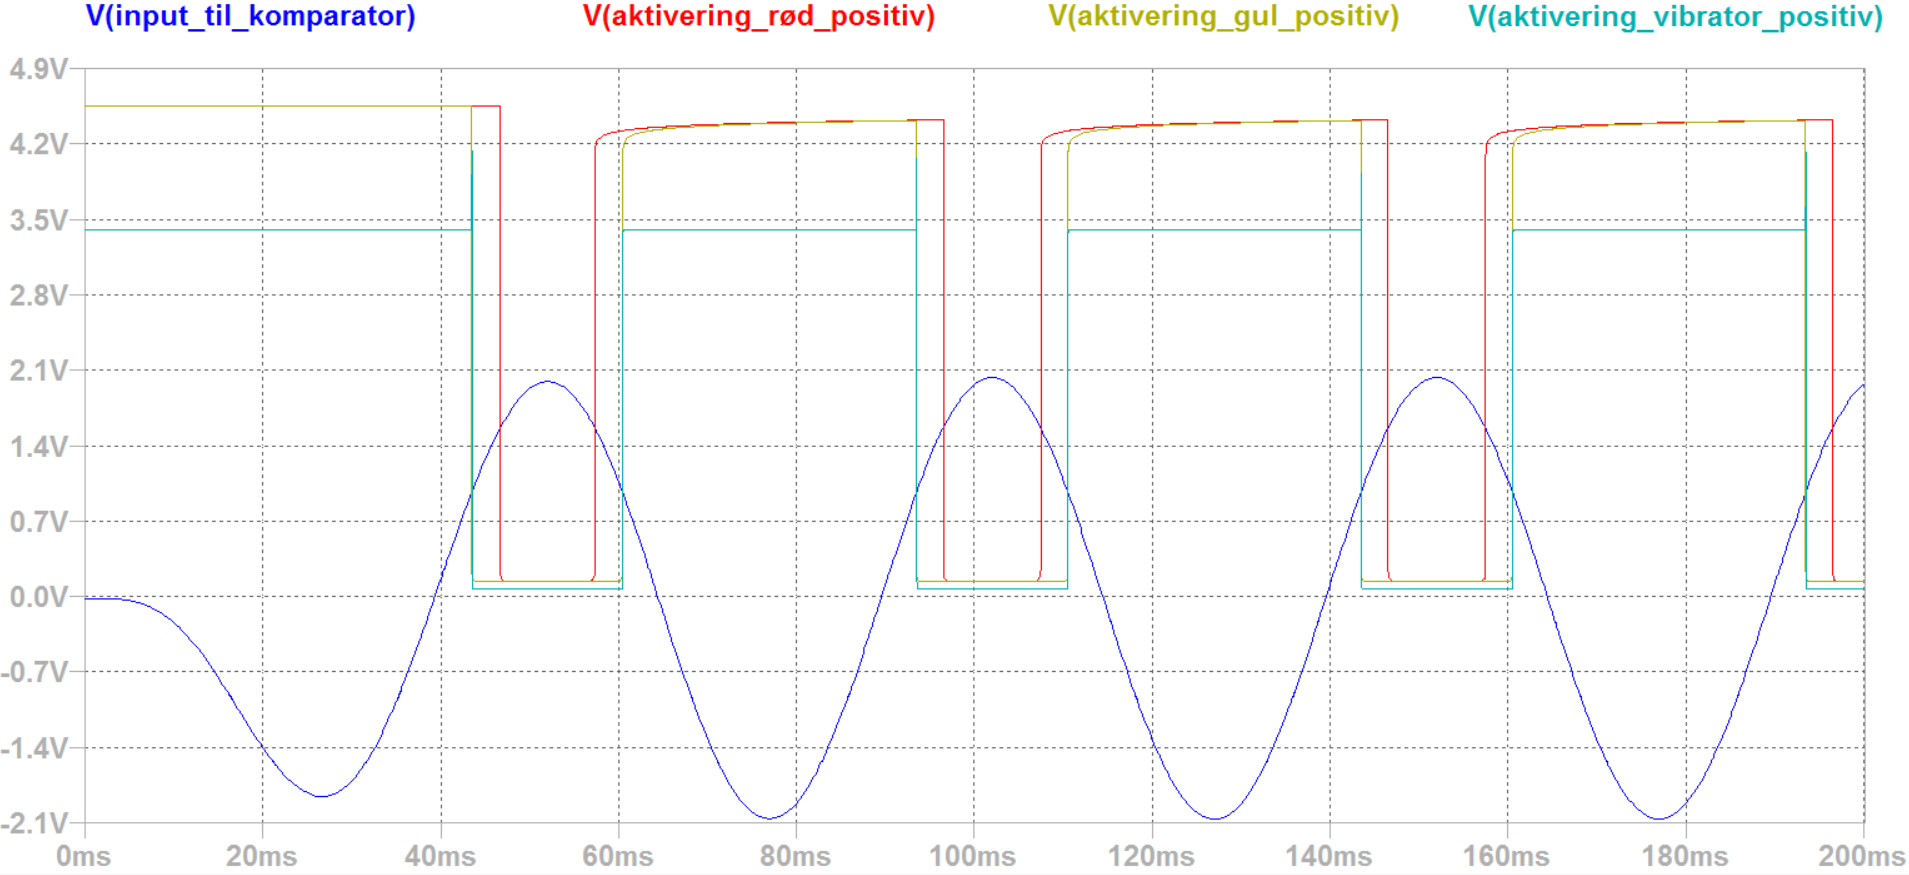
\includegraphics[scale=.38]{figures/cProblemloesning/Samlet_system_sim3.PNG}
	\caption{På figuren ses inputtet til komparatorblokken plottet sammen med visualiseringen af, hvornår LED'erne samt vibratorerne i positiv retning aktiveres. Der ses, at den røde LED aktiveres, når inputsignalet er over ca. $1.5$V. Den gule LED samt vibratoren i positiv retning aktiverer, når inputsignalet er ca. $0.9$V.}
	\label{fig:samlet_system_sim2}
\end{figure}
\begin{figure}[H]
	\centering
	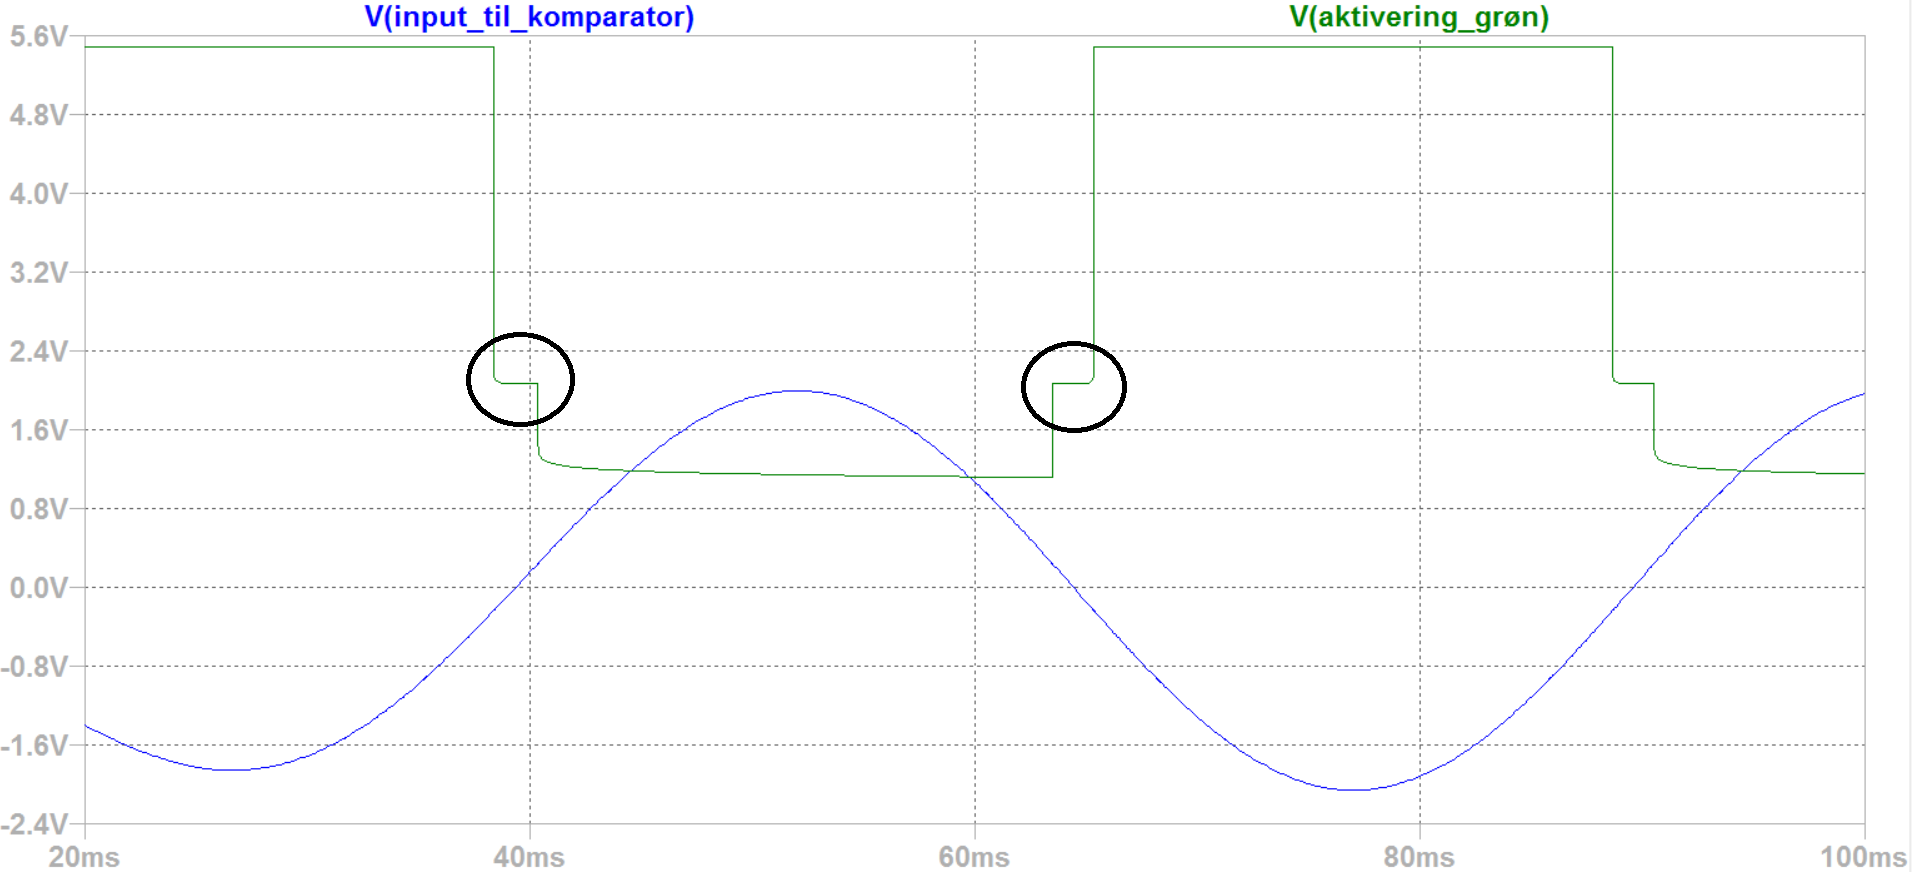
\includegraphics[scale=.38]{figures/cProblemloesning/Samlet_system_sim5.PNG}
	\caption{På figuren ses inputtet til komparatorblokken plottet sammen med visualiseringen af, hvornår den grønne LED er aktiveret. Det ses, at den grønne LED er designet i en vindueskonfiguration, hvilket betyder, at den kun er aktiv i hakket, som er markeret med to sorte cirkler på figuren. Det fremgår, at den er aktiv imellem $0.2$ - -$0.2$V.}
	\label{fig:samlet_system_sim5}
\end{figure}
\begin{figure}[H]
	\centering
	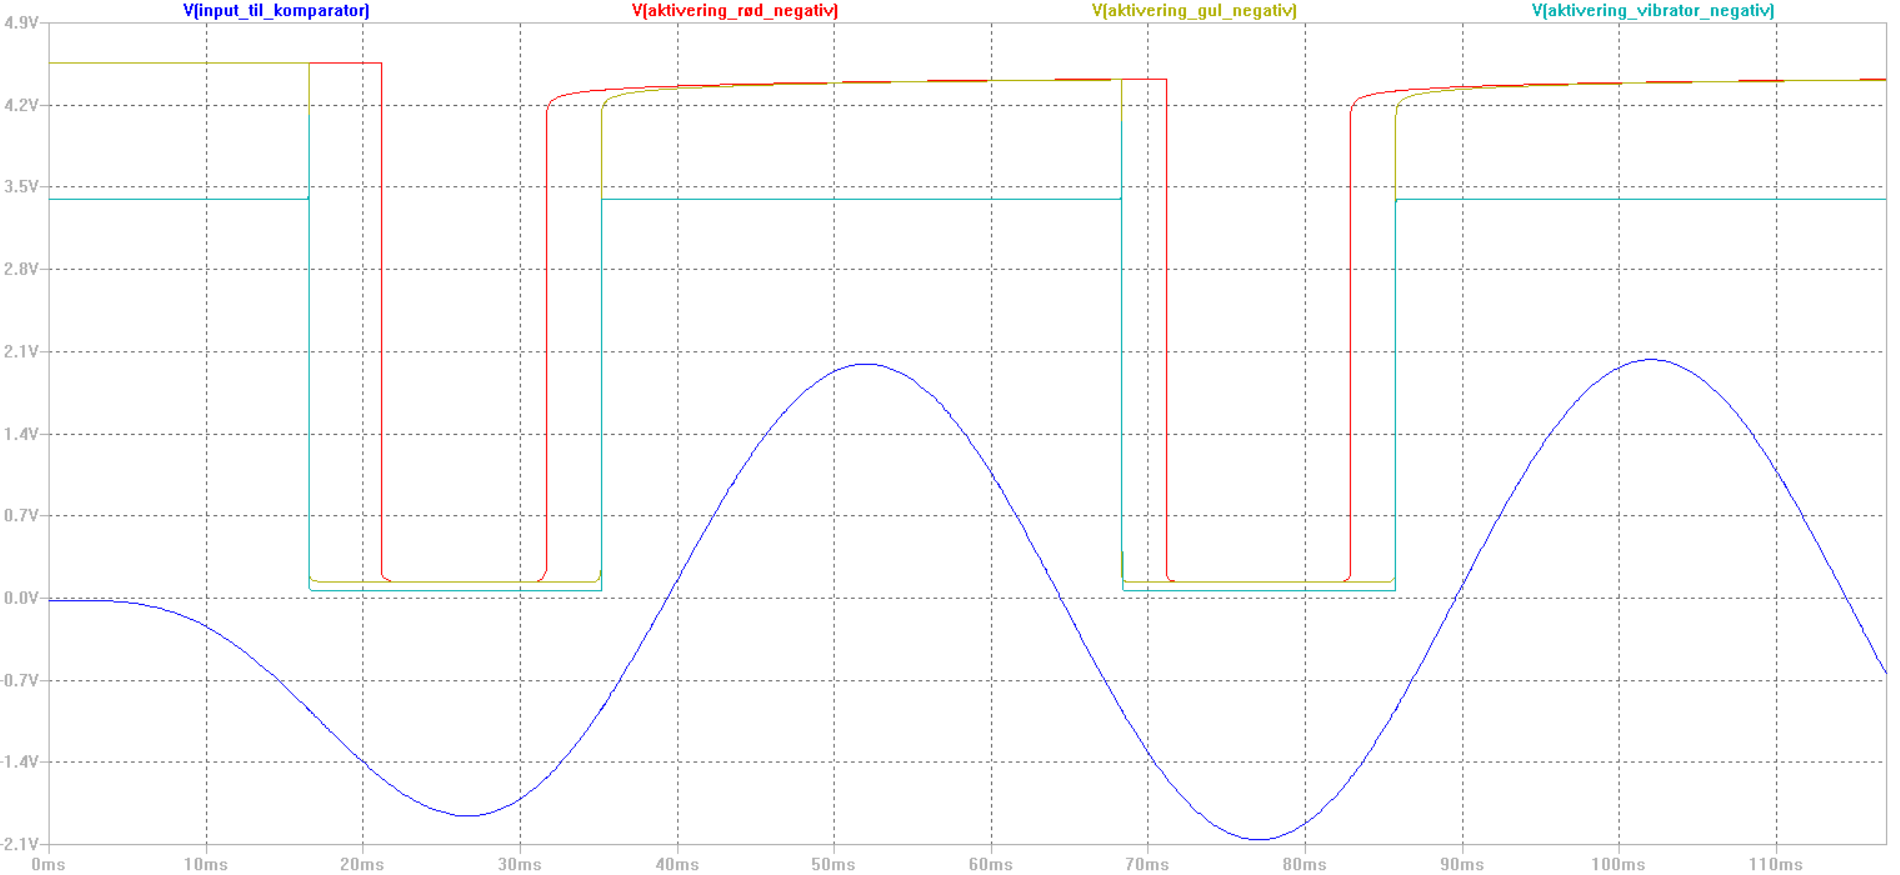
\includegraphics[scale=.38]{figures/cProblemloesning/Samlet_system_sim4.PNG}
	\caption{På figuren ses inputtet til komparatorblokken plottet sammen med visualiseringen af, hvornår LED'erne samt vibratorerne i negativ retning aktiveres. Der ses, at den røde LED aktiverer, når inputsignalet er over ca. -$1.5$V. Den gule LED samt vibratoren aktiverer, når inputsignalet er ca. -$0.9$V.}
	\label{fig:samlet_system_sim3}
\end{figure}
\noindent Ifølge figurerne og de grove aflæsninger aktiveres LED'erne samt vibratorerne ved de korrekte tærskelværdier. Der aflæses igennem LTspice, hvad outputtet er fra accelerometret ved aktivering af de enkelte feedbackkomponenter. Dette ses i \tableref{tab:samlet_sim}:
\begin{table}[H]
	\centering
	\begin{tabular}{l|l|l|l|}
		\cline{2-4}
		\textit{}                                                                                              & \textit{\begin{tabular}[c]{@{}l@{}}Output fra\\ accelerometer\end{tabular}} & \textit{\begin{tabular}[c]{@{}l@{}}Graders\\ hældning\end{tabular}}          & \textit{\% afvigelse}                                      \\ \hline
		\multicolumn{1}{|l|}{\textit{\begin{tabular}[c]{@{}l@{}}Rød LED\\ positiv\end{tabular}}}               & $1.6763$V                                                                   & $11.84^{\circ}$                                                              & $8.92\%$                                                   \\ \hline
		\multicolumn{1}{|l|}{\textit{\begin{tabular}[c]{@{}l@{}}Gul LED\\ \& vibrator\\ positiv\end{tabular}}} & $1.6620$V                                                                   & $7.97^{\circ}$                                                               & $0.38\%$                                                   \\ \hline
		\multicolumn{1}{|l|}{\textit{Grøn LED}}                                                                & \begin{tabular}[c]{@{}l@{}}$1.6400$V\\ $1.6251$V\end{tabular}               & \begin{tabular}[c]{@{}l@{}}$2.03^{\circ}$ til\\ -$2.06^{\circ}$\end{tabular} & \begin{tabular}[c]{@{}l@{}}$1.5\%$ \&\\ $3\%$\end{tabular} \\ \hline
		\multicolumn{1}{|l|}{\textit{\begin{tabular}[c]{@{}l@{}}Gul LED\\ \& vibrator\\ negativ\end{tabular}}} & $1.6027$V                                                                   & -$8.27^{\circ}$                                                              & $3.4\%$                                                    \\ \hline
		\multicolumn{1}{|l|}{\textit{\begin{tabular}[c]{@{}l@{}}Rød LED\\ negativ\end{tabular}}}               & $1.5843$V                                                                   & $13.38^{\circ}$                                                              & $2.9\%$                                                    \\ \hline
	\end{tabular}
	\caption{I tabellen ses resultatet af det simulerede samlede system ved aktivering af de enkelte feedbackkomponenter og den procentvise afvigelse fra de definerede hældningsgrader.}
	\label{tab:samlet_sim}
\end{table}

\subsection{Implementering og test}
Det samlede system implementeres på to breadboards. Opsætningen kan ses på \figref{fig:samlet_system_real}
\begin{figure}[H]
	\centering
	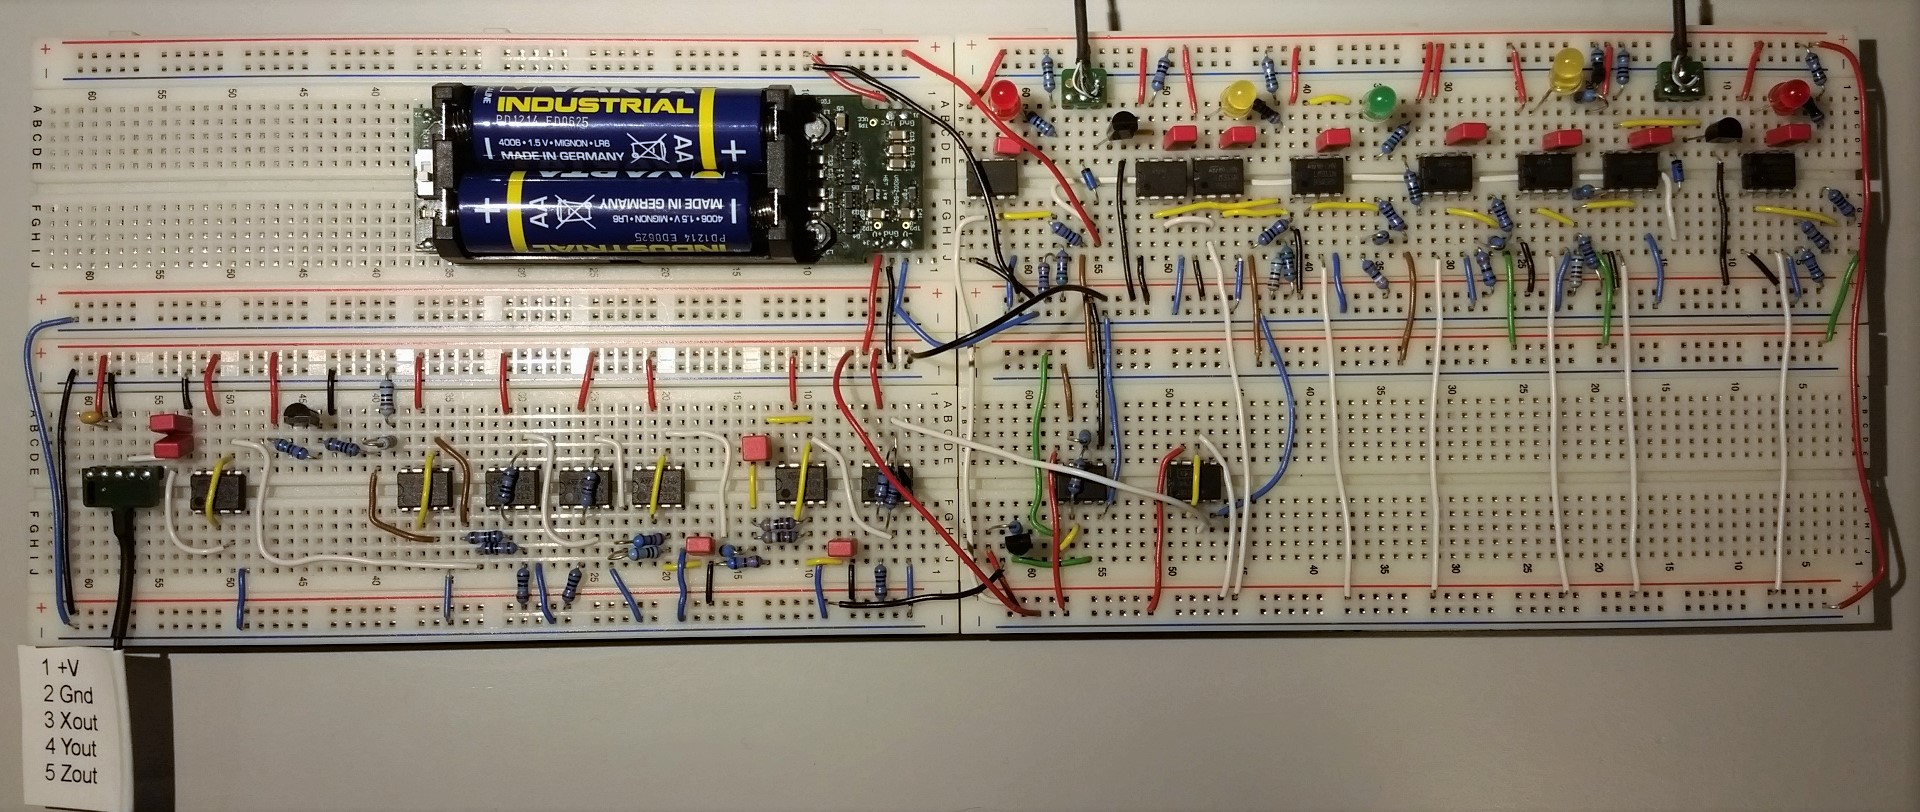
\includegraphics[scale=.22]{figures/cProblemloesning/Samlet_system2.jpg}
	\caption{På figuren ses implementeringen af systemet. Ledningernes farve symboliserer forskellige ting: De hvide leder signalet fra accelerometret igennem systemet og de røde og blå leder hhv. den positive og negative strømforsyning til de forskellige komponenter i systemet. De sorte ledninger leder til ground, og de gule ledninger fungerer som forbindelsesveje. De grønne og brune ledninger leder hhv. en positiv og negativ referencespænding til offsettet og komparatorerne.}
	\label{fig:samlet_system_real}
\end{figure}
\noindent Herefter kan det samlede system blive testet. Systemet vil blive testet på to forskellige måder - først en test efter samme principper som i testen af accelerometeret og efterfølgende en test af det digitale output. \\

\noindent I testen af det samlede system tages der udgangspunkt i principperne fra testen af accelerometeret beskrevet i afsnit \ref{Acc_afsnit} på side \pageref{Acc_afsnit}. Det måles, hvorvidt systemet opfylder de overordnede funktionelle krav jævnfør afsnit \ref{FunkKrav} på side \pageref{FunkKrav}, ved at hælde accelerometeret i positiv og negativ retning indtil udløst feedback og ved disse tidspunkter aflæse outputtet fra accelerometeret på et multimeter.
\subsubsection{Test 1}
Ved test af den analoge del af systemet måles spændingsfaldet over LED'erne og vibratorerne før og efter aktivering. Derudover måles outputtet fra accelerometret lige ved aktivering af de forskellige komponenter. Disse målinger foretages med et multimeter. Resultatet fremgår af \tableref{Tab:resultat:test1a}:
\begin{table}[H]
	\centering
	\begin{tabular}{l|l|l|l|}
		\cline{2-4}
		\textit{}                                                                                 & \textit{\begin{tabular}[c]{@{}l@{}}Spændingsfald over \\ komponent før\\ udløst feedback\end{tabular}} & \textit{\begin{tabular}[c]{@{}l@{}}Output fra\\ accelerometer\\ ved udløst feedback\end{tabular}} & \textit{\begin{tabular}[c]{@{}l@{}}Spændingsfald over\\ komponent efter \\ udløst feedback\end{tabular}} \\ \hline
		\multicolumn{1}{|l|}{\textit{\begin{tabular}[c]{@{}l@{}}Rød LED\\ negativ\end{tabular}}}  & $1.3296$V                                                                                         & $1.5822$V                                                                                    & $2.0324$V                                                                                           \\ \hline
		\multicolumn{1}{|l|}{\textit{\begin{tabular}[c]{@{}l@{}}Vibrator\\ negativ\end{tabular}}} & $0.6$mV                                                                                           & $1.6005$V                                                                                    & $2.9995$V                                                                                           \\ \hline
		\multicolumn{1}{|l|}{\textit{\begin{tabular}[c]{@{}l@{}}Gul LED\\ negativ\end{tabular}}}  & $1.4310$V                                                                                         & $1.6005$V                                                                                    & $2.0700$V                                                                                           \\ \hline
		\multicolumn{1}{|l|}{\multirow{2}{*}{\textit{Grøn LED}}}                                  & \multirow{2}{*}{$1.4611$V}                                                                        & $1.6243$V                                                                                    & \multirow{2}{*}{$2.0196$V}                                                                          \\ \cline{3-3}
		\multicolumn{1}{|l|}{}                                                                    &                                                                                                   & $1.6377$V                                                                                    &                                                                                                     \\ \hline
		\multicolumn{1}{|l|}{\textit{\begin{tabular}[c]{@{}l@{}}Gul LED\\ positiv\end{tabular}}}  & $1.4247$V                                                                                         & $1.6562$V                                                                                    & $2.1187$V                                                                                           \\ \hline
		\multicolumn{1}{|l|}{\textit{\begin{tabular}[c]{@{}l@{}}Vibrator\\ positiv\end{tabular}}} & $0.1$mV                                                                                           & $1.6562$V                                                                                    & $3.1029$V                                                                                           \\ \hline
		\multicolumn{1}{|l|}{\textit{\begin{tabular}[c]{@{}l@{}}Rød LED\\ negativ\end{tabular}}}  & $1.3311$V                                                                                         & $1.6740$V                                                                                    & $2.0605$V                                                                                           \\ \hline
	\end{tabular}
	\caption{I tabellen ses resultatet fra målingerne af den analoge del af systemet.}
	\label{Tab:resultat:test1a}
\end{table}
\noindent Der ses i \tableref{Tab:resultat:test1a}, at der forekommer et spændingsfald over LED'erne, selvom de ikke afgiver synligt lys. Dette skyldes, at der løber en lækstrøm igennem dem, men denne er ikke tilstrækkelig for aktivering af synligt lys. På \figref{fig:samlet_system_LED} ses graferne for forholdet imellem spændingsfaldet over LED'erne og strømmen, der løber igennem, for de enkelte LED'er. \cite{kingbright}
\begin{figure}[H]
	\centering
	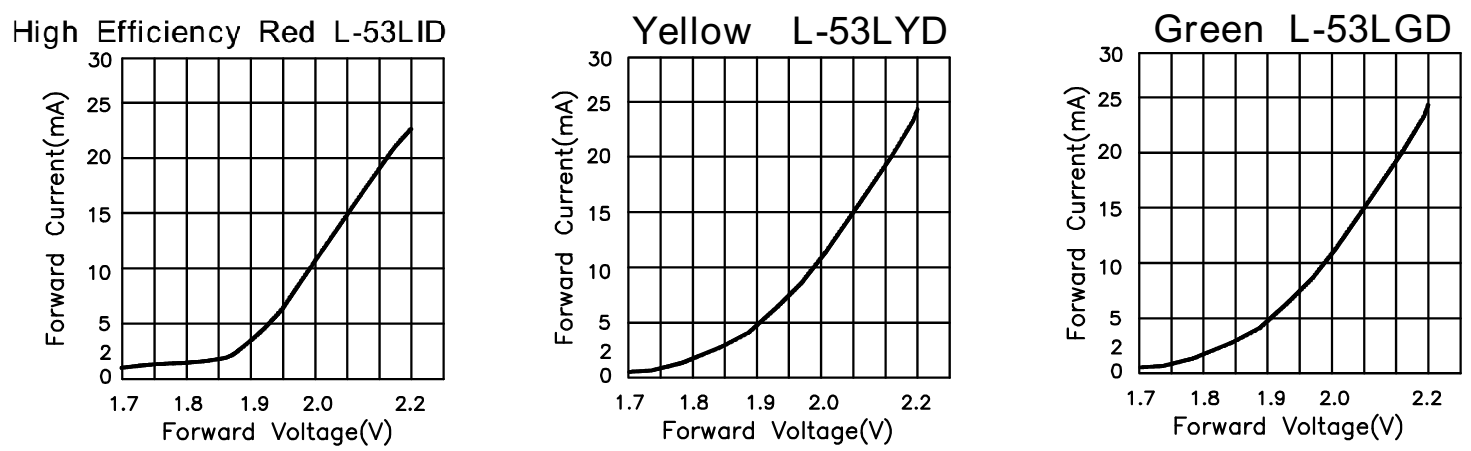
\includegraphics[scale=.45]{figures/cProblemloesning/Samlet_system_LED.PNG}
	\caption{På figuren ses der tre grafer for hhv. den røde, gule og grønne LED. Graferne viser forholdet imellem spændingsfaldet over LED'erne og strømmen, der løber igennem, for de enkelte LED'er. \textit{(Revideret)} \cite{kingbright}}
	\label{fig:samlet_system_LED}
\end{figure}
\noindent Ifølge databladet for LED'erne vil de aktiveres ved $0.8$mA. Da der ikke er et lineært forhold imellem spændingsfaldet og strømmen på \figref{fig:samlet_system_LED}, er det ikke muligt at vurdere, om LED'erne faktisk er aktiverede ved målingerne i anden kolonne i \tableref{Tab:resultat:test1a}. Jævnfør afsnit \ref{Afs_Komparator} på side \pageref{Afs_Komparator} skal en LED modtage $20$mA for at afgive tydeligt lys. Da komparatorkonfigurationen er tilpasset til, at denne strøm skal løbe over LED'erne, kan det forventede spændingsfald aflæses på grafernes x-akse for de enkelte LED'er. Ud fra disse værdier beregnes afvigelsen for de målte spændingsfald. \\
I fjerde kolonne på \tableref{Tab:resultat:test1a} ses det målte spændingsfald, når der teoretisk løber $20$mA over LED'en. De beregnede afvigelser ses i \tableref{tab:samlet_procent1a}. De teoretiske værdier for spændingsfaldet er aflæst på x aksen ud fra $20$mA på y aksen på \figref{fig:samlet_system_LED}.
\begin{table}[H]
	\centering
	\begin{tabular}{l|l|l|l|}
		\cline{2-4}
		\textit{} & \textit{\begin{tabular}[c]{@{}l@{}}Teoretisk\\ spændingsfald\end{tabular}} & \textit{\begin{tabular}[c]{@{}l@{}}Målte\\ spændingsfald\end{tabular}} & \textit{\% afvigelse} \\ \hline
		\multicolumn{1}{|l|}{\textit{\begin{tabular}[c]{@{}l@{}}Rød LED\\ negativ\end{tabular}}} & $2.14$V                                                                    & $2.0324$V                                                              & $5.03\%$              \\ \hline
		\multicolumn{1}{|l|}{\textit{\begin{tabular}[c]{@{}l@{}}Gul LED\\ negativ\end{tabular}}} & $2.15$V                                                                    & $2.0700$V                                                              & $3.73\%$              \\ \hline
		\multicolumn{1}{|l|}{\textit{Grøn LED}}                                                  & $2.14$V                                                                    & $2.0196$V                                                              & $5.63\%$              \\ \hline
		\multicolumn{1}{|l|}{\textit{\begin{tabular}[c]{@{}l@{}}Gul LED\\ positiv\end{tabular}}} & $2.15$V                                                                    & $2.1187$V                                                              & $1.46\%$              \\ \hline
		\multicolumn{1}{|l|}{\textit{\begin{tabular}[c]{@{}l@{}}Rød LED\\ negativ\end{tabular}}} & $2.14$V                                                                    & $2.0605$V                                                              & $3.71\%$              \\ \hline
	\end{tabular}
	\caption{I tabellen ses procentafvigelsen fra det forventede spændingsfald ved aktivering af LED'erne.}
	\label{tab:samlet_procent1a}
\end{table}
Det fremgår af \tableref{tab:samlet_procent1a}, at der forekommer afvigelser imellem det målte og det forventede spændingsfald for alle LED'erne. Alle de målte værdier ligger under de forventede værdier, hvorfor det må forventes, at LED'ernes lys er svagere end forventet. Da det typiske interval for spændingsfaldet ved synligt lys ligger på $1.7$-$1.9$V og maksimalt på $2.0$-$2.2$V jævnfør afsnit \ref{Afs_Komparator} på side \pageref{Afs_Komparator}, vurderes det imidlertid, at LED'erne udløser deres feedback efter hensigten.\\
De benyttede vibratorer aktiveres, når der sker et spændingsfald over dem på $2.3$V. \cite{Machinery2009} Teoretisk bør der ikke forekømme spændingsfald over vibratorerne, når disse er slukkede. Ud fra målingerne i \tableref{Tab:resultat:test1a} vurderes det, at dette er gældende, da der arbejdes med reelle komponenter under implementeringen. Ved udløst feedback sker der et spændingsfald for begge vibratorer på ca. $3$V. Dermed er spændingsfaldet over grænsen for aktivering, og det vurderes derfor, at vibratorerne udløser deres feedback efter hensigten. \\
Ud fra de målte outputværdier fra accelerometeret kan det beregnes, om feedbackmekanismerne aktiveres ved de definerede hældningsgrader jævnfør afsnit \ref{KomparatorAfs} på side \pageref{KomparatorAfs}. Dette gøres ved at tage outputværdien, trække offsettet i accelerometret fra og derefter dividere dette med hhv. -$0.0036$V og $0.0037$V for output i negativ og positiv retning.
\begin{align}\label{eq:graderLED_1}
\dfrac{(1.5822 - 1.6325)}{-0.0036} = 13.97^{\circ}\text{ for aktivering af rød LED i negativ retning} \\
\dfrac{(1.6005 - 1.6325)}{-0.0036} = 8.89^{\circ}\text{ for aktivering af gul LED samt vibrator i negativ retning} \\
\dfrac{(1.6243 - 1.6325)}{-0.0036} = 2.28^{\circ}\text{ for deaktivering af grøn LED i negativ retning} \\
\dfrac{(1.6377 - 1.6325)}{0.0037} = 1.41^{\circ}\text{ for deaktivering af grøn LED i positiv retning} \\
\dfrac{(1.6562 - 1.6325)}{0.0037} = 6.41^{\circ}\text{ for aktivering af gul LED samt vibrator i positiv retning} \\ \label{eq:graderLED_2}
\dfrac{(1.6740 - 1.6325)}{0.0037} = 11.22^{\circ}\text{ for aktivering af rød LED i positiv retning}
\end{align}
\noindent Der ses i overstående ligninger, at der er en afvigelse i accelerometerets hældning ift. de definerede grader for aktivering af feedbacken. Grunden til dette kan være, at referencespændingen til offsettet måles til $1.6302$V, hvilket er -$0.0023$V fra det teoretiske offset i accelerometret. Derved forskydes offsettet, og graderne for hældning af accelerometret i negativ retning vil blive større, mens graderne vil blive mindre i positiv retning. Derudover skal der tages højde for afvigelserne i de enkelte blokke i systemet, som undervejs er blevet tolereret og accepteret. Disse vil tilsammen kunne skabe en større afvigelse for det samlede system. \\
På baggrund af målingerne og de vurderede fejlkilder godkendes den analoge del af systemet og det vurderes, at det virker efter hensigten ift. de overordnede funktionelle krav.\\

\subsubsection{Test 2}
Ved test af den digitale del af systemet undersøges det, hvorvidt systemet kan give et digitalt output, som kan aflæses og gemmes jævnfør afsnit \ref{FunkKrav} på side \pageref{FunkKrav}. \\
Ved testen roteres accelerometret i positiv og negativ retning, hvilket er afbilledet på \figref{fig:samlet_system_digital}:
\begin{figure}[H]
	\centering
	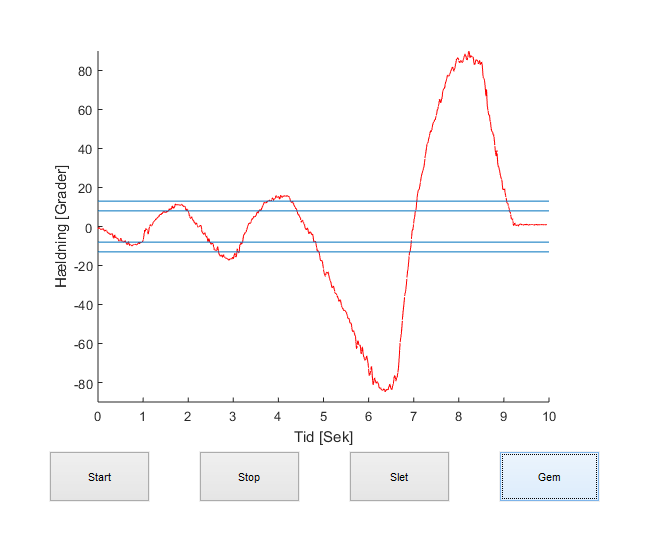
\includegraphics[scale=.6]{figures/cProblemloesning/Software.jpg}
	\caption{På figuren ses brugerfladen for programmet. De blå streger repræsenterer de definerede hældningsgrader, hvor der gives feedback i den analoge del. Den røde graf repræsenterer en måling foretaget med accelerometret. På x-aksen ses tiden og på y-aksen ses hældningsgrader af accelerometret.}
	\label{fig:samlet_system_digital}
\end{figure}
\noindent Det fremgår af \figref{fig:samlet_system_digital}, at det er muligt at aflæse den målte hældning af accelerometret på en graf samt at gemme målingen.\\
På baggrund af testen og \figref{fig:samlet_system_digital}  godkendes den digitale del af systemet og det vurderes, at det virker efter hensigten.